\section{Pancreatic Tissue Model} \label{ssec:panc_tis_mod}
 In this first attempt of modelization from scratch the main focus was put on reflecting only the main structural features on the virtual specimens. Given the pancreatic tissue's organization, described back in section \ref{ssec:pancr_anat}, the first features I decided to emphasize on were: 1) The iterative (with a fractal-like behavior) ramification of blood vessels for the irrigation of glandular acinus, 2) The space-filling distribution of acinus in the tissue, in fact, we expect a homogeneous density in the organ and to not see \textit{holes} at all inside it. In this section I will describe step by step all the process I followed to create the model of a portion of pancreatic tissue, and all the interesting pitfalls I overcame.

\subsection{2D Ramification}
    The first step was taken in two dimensions, and it was the choice of the right \textit{structure} to emulate the ramification of blood vessels in pancreatic tissue. The choice fell on a particular parametric L-system, as the one shown in Figure \ref{fig:bf_ls}, in section \ref{ssec:Lsys}. This structure is made of an iterative bifurcation of gradually shorter segments, with an angle of $\pm 85 \degree$ respect the main direction. For a start I added some features to give a more realistic look to the structure, which are all well represented in Figure \ref{fig:ram_feat}:

    \begin{figure}
        \centering
        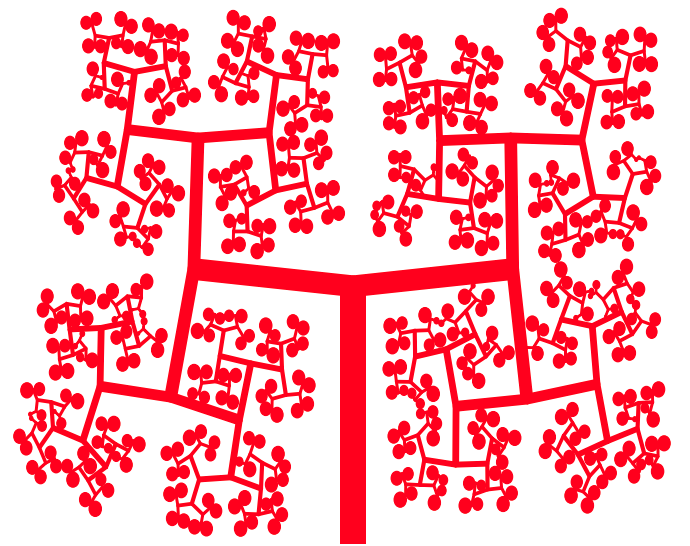
\includegraphics[width = 0.6\textwidth]{images/ram_feat}
        \caption{The development of the simple ramification in Figure \ref{fig:bf_ls}, with some features to give it a more realistic look, like progressive thickness, angular noise in bifurcation, and spheres at free ends of the ramification. The image is made using the tools exposed in section \ref{ssec:Lsys}.}
        \label{fig:ram_feat}
    \end{figure}

    \begin{itemize}
        \item A progressive thickness of the bifurcation's segments, starting from a thick main branch that dwindles every junction. The idea is that the main blood vessel becomes gradually smaller becoming capillaries for single-cell irrigation.
        \item A progressive randomness in the angular deflection at every fork. Perfectly repeated angles are almost nonexistent in nature, so I decided to introduce an increasing indetermination in the angle of bifurcation from the main branch to the free ends of the structures' branches.
        \item Spheres at the ends of each branch, which acts as glandular acini. The maximum radius is comparable to the length of the final segments.
        \item A mechanism to avoid self-superimposition between branches and spheres. After the insertion of noise, the cumulative effect on the final segments might lead to different branches to intersect. This is clearly a paradoxical situation, as real tissues while growing naturally occupy the space in a gradual way.
    \end{itemize}

    To produce the specific image in Figure \ref{fig:ram_feat} I used a particular setting of the tool described in section \ref{ssec:Lsys}, which has a greatly wider range of customization and could be used to create many other different structures to the need.

\subsection{Expansion to 3D}
    The successive step I followed was to expand this structure in three dimensions and fill the space in each of the three directions. The idea to evolve the structure in Figure \ref{fig:ram_feat} is simply to twist of 90$\degree$ the ramification at every junction point, in such a way to exit the previous belonging plane. However, putting into practice this development has not been easy. The organization of the structure in a 3D space requires an appropriate system of reference for handling subsequent rotations in three dimensions. The best option for handling relative 3D rotations, often used in computer graphics and every kind of 3D modelization, are quaternions, as shown in section \ref{ssec:quat}.

    \begin{figure}
        \centering
        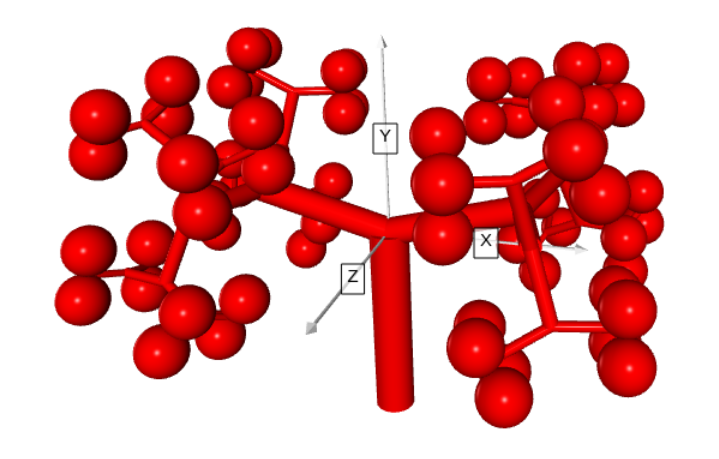
\includegraphics[width = 0.6\textwidth]{images/3d_ram}
        \caption{The three-dimensional expansion of the 2D ramification in Figure \ref{fig:ram_feat}.}
        \label{fig:3d_ram}
    \end{figure}

    In this new structure, segments are replaced with cylinders, and circles are replaced with spheres. At every bifurcation to every cylinder are applied the following transformations:
    \begin{itemize}
        \item a contraction in its extensions, regulated by an adjustable parameter $R$.
        \item the usual deviation of $\pm 85 \degree$ respect to the direction of the parent branch.
        \item a 90$\degree$ specific rotation along the axis of its parent branch.
    \end{itemize}

    The result of this procedure is a 3D ramification like the one in Figure \ref{fig:3d_ram}, in which we can recognize a good coverage of the space defined by the structure's boundaries and immediate relation with the 2D structure in Figure \ref{fig:ram_feat}. It should be noted that, in the further refinements of the model from now on, there won't be present the progressive angular indetermination on the direction of branches. Although it is a feature already implemented and working, it requires efficient control to avoid reciprocal overlapping between elements to produce a realistic structure. This second element has not been already developed and it would certainly enrich the representative power of the model.

    As for the 2D ramification the production of this structure has required the implementation of a tool for the 3D generation with a greatly wider power, able to produce almost any type of three-dimensional iterative structure after the right adjustment, and with a high degree of customization. It is necessary to mention the fundamental tool which allowed me to accomplish this step of the development, which is the \texttt{Python} library \texttt{VPython}: a library for 3D graphics visualization. This library allows a convenient and powerful interface to draw many types of objects and to move them around in space, which has been priceless to orient my self in three dimensions while developing the model and to produce all the 3D images visible in this work.

\subsection{Subdivision in Cells}
    Once the 3D backbone of the pancreatic tissue blood vessels ramification system has taken shape, the next step was to embed all this structure in a spatial partitioning process, to create the subdivision into single cells. To perform this important task I used a 3D Voronoi decomposition, as shown in section \ref{ssec:vor_tass}. Depending on the choice of the starting points, the Voronoi tessellation could be an excellent item to recreate individual cells because it could guarantee some important properties: all the regions are convex, adjacent, with similar size and volume, with different shapes, and without holes. These have been chosen as the most significant properties to be reflected in the first modelization of cells.

    As shown in section \ref{ssec:vor_tass}, the Voronoi decomposition strongly depends on the choice of the starting point. Points spread uniformly on a 3D regular lattice will produce a series of parallelepipeds repeated in the space. An example of uniform tessellation is shown in Figure \ref{fig:reg_vor}. On the other hand, a decomposition based on a quasi-random generated point can present all the good properties we mentioned before, including the diversity in shapes. In Figure \ref{fig:sal_vor} is shown an example of a Voronoi decomposition based on points sampled in a 3D with the Saltelli algorithm, in reference to section \ref{ssec:saltelli}. Regardless of the points sampling technique, the boundaries of the sampling 3D box have been chosen to loosely contain the ramification.

    \begin{figure}
        \centering
        \begin{subfigure}[b]{0.45\textwidth}
             \centering
             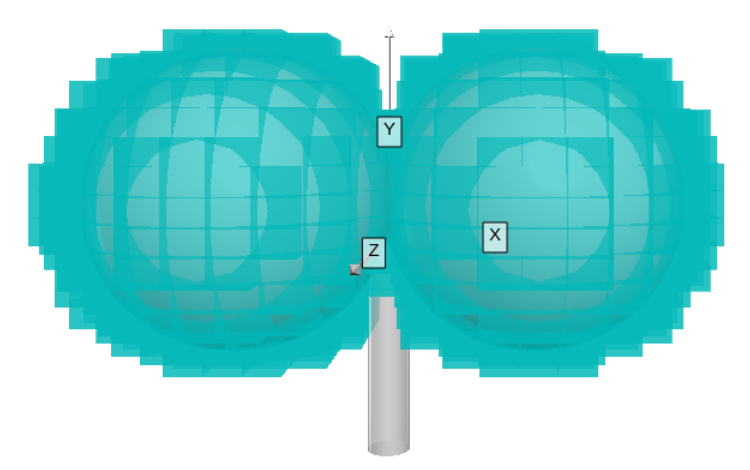
\includegraphics[width = \textwidth]{images/reg_vor}
             \caption{Regular lattice.}
             \label{fig:reg_vor}
        \end{subfigure}
        \hfill
        \begin{subfigure}[b]{0.45\textwidth}
             \centering
             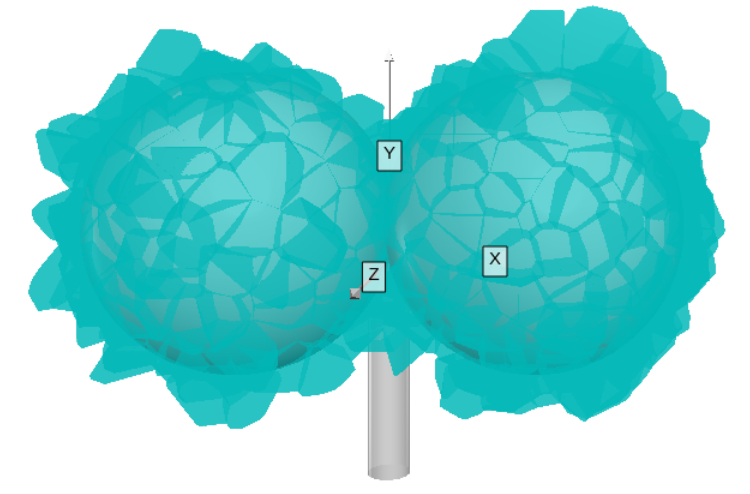
\includegraphics[width = \textwidth]{images/sal_vor}
             \caption{Sampling with Saltelli algorithm.}
             \label{fig:sal_vor}
        \end{subfigure}
        \caption{Comparison between two Voronoi decompositions. The first (left) is created from a regular lattice of starting points, and every piece is exactly equal to all the others, creating a regular subdivision of the space. The second (right) is created instead from a sampling made following the Saltelli quasi-random algorithm. The pieces are all different in shape, but they all have similar sizes and volumes. In this pictures in particular have been shown only the pieces of the tessellation which lie in correspondence to the boundaries of the spheres underneath. While watching this picture one should immagine the decomposition extended similarly in all the space around the ramification, within certain boundaries, which loosely contains the structure. This limitation was necessary to enhance the interpretability of the image. }
        \label{fig:vor_comp}
    \end{figure}

    There are tough some delicate considerations to be highlighted about the decomposition procedure. The first regards the most external pieces of the decomposition. Whilst the internal pieces are neatly bounded and defined, the most external layer instead is made on unbounded regions, which extend themselves to infinity. Those regions have clearly to be rejected, as it would be absurd for a cell to have an infinity volume. Typically those unbounded regions are resized in order to adhere to some limiting boundaries, with an operation known as \textit{cropping}. In Figure \ref{fig:crop_vor} is shown an example of circular cropping in a 2D Voronoi decomposition: all the regions which intersect the circumference have to be resized.

    \begin{figure}
        \centering
        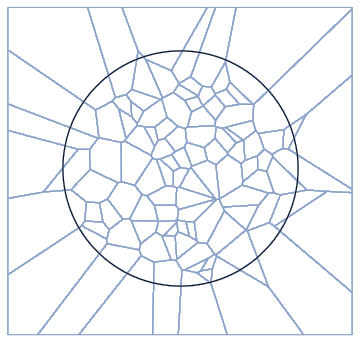
\includegraphics[width = 0.5\textwidth]{images/crop_vor}
        \caption{Example of circular cropping in a 2D Voronoi decomposition: all the regions which intersect the circumference have to be resized.}
        \label{fig:crop_vor}
    \end{figure}

    The cropping operation in 3D is extremely complex, tough. Thus, a more simple and efficient, yet less elegant, technique has been used. Instead of resizing the regions which lie on the boundaries of the sampling region, those regions have directly been rejected. This process is really fast and it does not lead to any danger of representativity loss if the boundaries are loose enough and if the density of sampling is not too low.

    The other important consideration regards the density of sampling points. Increasing the number of points to be extracted from the same volume automatically the number of cells in the box will rise, and in contrast, their relative dimension will decrease. This is a key element of the model: a too rarified decomposition would not bee able to reflect the complexity of the structure underneath, but a too crowd decomposition on the other side would lead to an unrealistic dimension of the cells in the tissue. Furthermore, this parameter has a huge influence on the computing time necessary to generate the model and to process it for the sectioning as will be shown in section \ref{sec:synth_image}. In almost all the applications so far, the density parameter has been tuned by eye, with a trial and error procedure. Although, a more rigorous way to adjust this parameter would be to consider the average dimension of the cells and make some microanatomical considerations to define the correct relative dimensions. The measure of the volume\footnote{The volume is expressed in the same arbitrary length unit of measures used during the ramification structure. This allows a coherent reference tool.} of the decomposition's regions is an accessible parameter, thus an easy way to estimate the average linear dimension of the cells can be to approximate all the cells to cuboid seeing their volumes as $V \approx L^3$. Averaging all the $L$ measures an estimate $\hat{L}$ can be done. This average length may be compared to the length of the blood vessel ramification, allowing a good reference tool.

\subsection{Cells Identity Assignment}
    The great power of creating all the models virtually is to know exactly the identity of every point in the structure. Although, This identity has to be reflected at the cellular level, assigning to every region a label. Imagining the Voronoi decomposition represented in Figure  \ref{fig:sal_vor} extended to the entire box containing the ramification, good discrimination would distinguish three classes of cells: those which lie completely inside a sphere, those which lie completely outside a sphere, and those which lie on the boundaries of a sphere. In Figure \ref{fig:cell_id} is shown a portion of the complete decomposition where the three classes of cells are reported with different colors: the internal cells in red, those on the boundaries in turquoise, and the external cells in gray.

    \begin{figure}
        \centering
        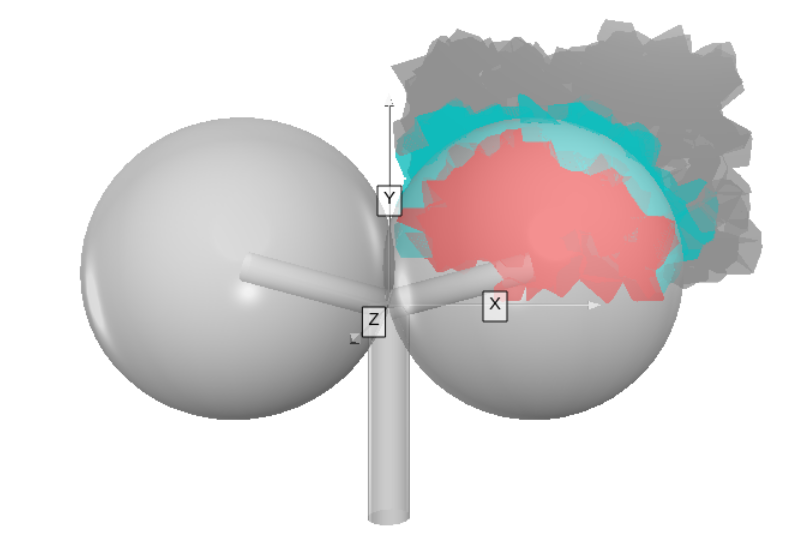
\includegraphics[width = 0.5\textwidth]{images/cell_id}
        \caption{Portion of the complete Voronoi decomposition, showing the three different classes of cell in three different colors: the internal cells in red, those on the boundaries in turquoise and the external cells in gray.}
        \label{fig:cell_id}
    \end{figure}

    In this particular case to find the relative position between every sphere in the structure and each cell it has been used a test on the proximity between the spheres' centers and the vertices of every polyhedral cell. If all the vertices of a region lie within a distance lower than the radius from the center of the same sphere then that region can be said to be an internal one. If none of the vertices lie within the radius distance from any center then that region is said to be external. In any other case, the region is said to be on the boundaries of some sphere, and this third label is assigned to it. As could be imagined the number of cells inside the volume can grow very quickly, and in the more rich ramifications also the number of spheres could be high. If we think that any polyhedron has a number of vertices of the order of $20/30$ then it is clear that the number of distance evaluations could grow very quickly, requiring some relevant computational power in the more extended simulations. In order to optimize this computation, I decided to use a python implementation of a K-dimensional Tree, which is a space-partitioning data structure especially suited for fast and optimized computation of distances \cite{10.1145/361002.361007}. A K-d Tree is an algorithm that iteratively binary splits the space: every node of the three could be thought as a splitting $(k-1)$-hyperplane dividing the space into two semi-hyperspace. The result is an optimized algorithm for repeated distance evaluations. As for many other tools, in my code I used a pre-implemented module \texttt{KDTree} from the \texttt{Scipy} library.

    This procedure of labeling the regions is completely customizable, and it should be adapted to the specific application. By the way, the principle will always be to perform some sort of spatial consideration respect to the primary structure and assign all the interesting labels accordingly to the cells in the volume.

    After labeling the cells in the decomposition the model is considered complete. Every enrichment to the structure should be reflected in some type of label for the cells, which are chosen as the fundamental unit in the model. As we will see in section \ref{sec:synth_image} during the sectioning process in the produced image will be printed mainly the identity of the cells, hence any detail on a finer scale in the model would not be conveyed properly on the final image.

\section{Dermal Tissue Model} \label{ssec:derm_tis_mod}
    The modeling of the dermal tissue has followed analogous schedule respect to the previous model, hence many procedures and considerations have been repeated. The main target for this model was to recreate the stratification of different specific tissues in the section of a dermal sample. As clearly visible in Figure \ref{fig:derm_descr} in a dermal histological specimen one can distinguish the lighter and wider region of proper \textit{dermal} tissue, underneath a more shallow and darker region of \textit{epidermal} tissue. It is very interesting the boundary between those two regions, which can be seen as an irregular and smooth surface, populated of dermal lobes. On the other side of the epidermal layer lies a layer of \textit{keratin}, with a smooth and regular boundary surface. Keratin is a family of fibrous structural proteins known as scleroproteins, a key structural material for hair, nails, and the outer layer of skin. The upper white region in Figure \ref{fig:derm_descr} instead is the support for the samples to perform optical analysis, and has no histological meaning.

    \begin{description}
        \item [1) Stratificated Structure] \hfill \\
        In order to represent faithfully the stratification of different tissue layers, I decided to use one flat plane to separate epidermal tissue and the keratine layer and two boundary surfaces modulated by a Perlin noise function on different scales for the other two separations, as shown in Figure \ref{fig:2_surf_plot}. As stated in section \ref{ssec:perlin}, after some easy customization the generation of different Perlin noise surfaces is easy and straightforward. By the way, to achieve the regularity and the smoothness of the orange surface in Figure \ref{fig:2_surf_plot} it was needed a horizontal stretching.

        \begin{figure}
            \centering
            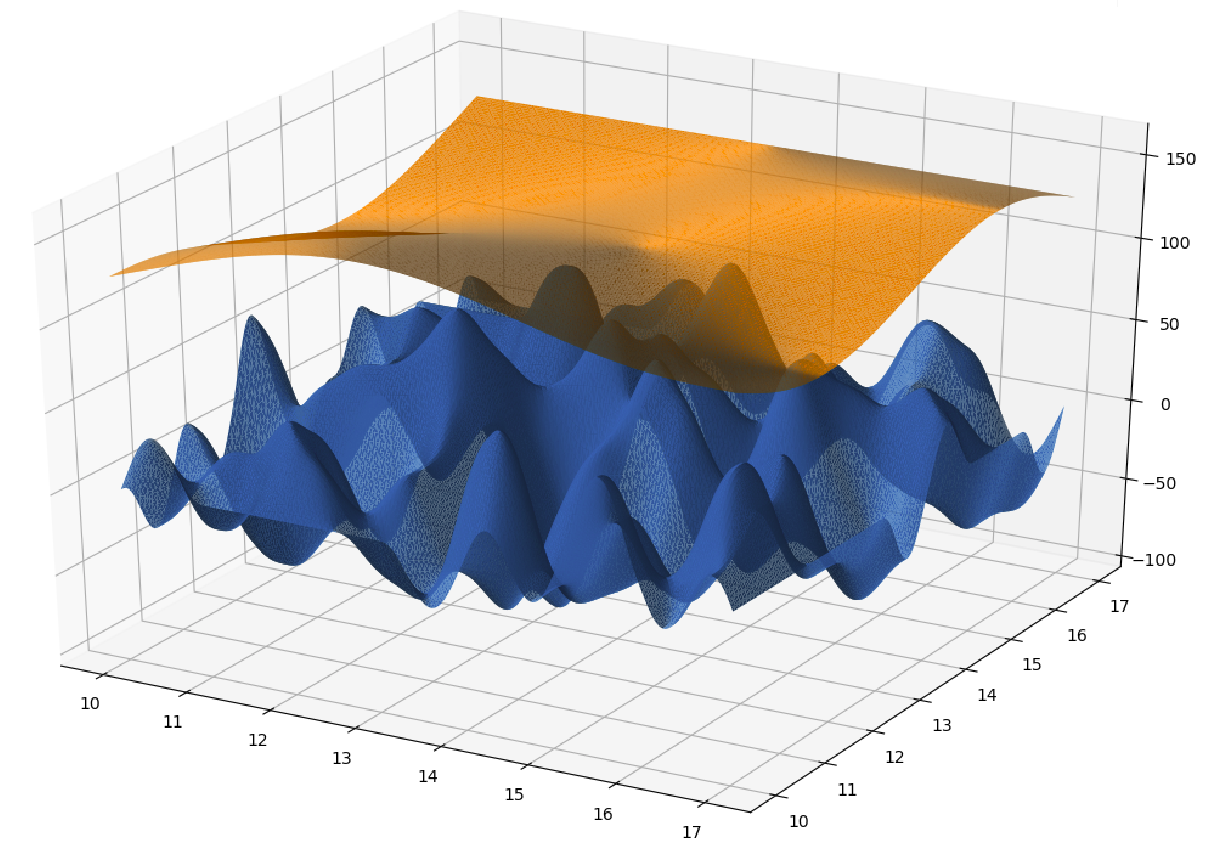
\includegraphics[width = 0.6\textwidth]{images/2_surf_plot}
            \caption{Pictures of two different Perlin noise surfaces used to separate dermal from epidermal tissue (blue) and epidermal from keratine layer (orange). The two surface are made by the same Perlin noise function, but the latter is stretched and compressed in order to have a more regular behavior.}
            \label{fig:2_surf_plot}
        \end{figure}

        Following the scale of the image, the standard blue surface is created in a $7 \times 7$ square, while the orange surface has primarily been generated in a $1 \times 1$ square, and then has been stretched to cover the same $7 \times 7$ square, multiplying the values in its grid points respectively for the stretching factors $R_x=R_y=\frac{1}{7}$. In this primary structure, there are many important parameters defining the surfaces, like the distance between the two surfaces' average values and the amplitudes of the peaks and the valleys of the surfaces. In its standard version the Perlin noise covers the $[-1;1]$ range, but with a simple multiplication for an amplitude factor $A_S$ the values can be adjusted. Those particular values have been adjusted after some tries to recreate the proportions typical of a real specimen. To sum up, each one of the two surfaces is stored as a discretized three-dimensional array, or better as an array of 3-tuples in the form $(x,y,f_{(x,y)})$, one tuple for every $(x,y)$ node of the grid, while the discretization grid was the same for both the surfaces.

        \item [2) Subdivison in Cells] \hfill \\
        The subdivision in cells of the volume containing the structure has followed the exact same steps described in section \ref{ssec:panc_tis_mod}, hence in this paragraph I will shortly resume the process. The first step is the definition of a suitable volume containing the structure. Then is the time for the generation of the decomposition's starting points according to a quasi-random number generation technique, as described in section \ref{ssec:saltelli}. Afterward, the points are used as a base for the decomposition, and all the cells with undefined boundaries are rejected

        \item [3) Cells Identity Assignment] \hfill \\
        The identity assignment procedure instead has been customized for this particular application. In this model there are no \textit{boundary} cells like the one lying on the spherical surfaces in the pancratic model, thus there is no need for a test on the position of each vertex of every cell. In this model, the starting point for every Voronoi region has been used as a reference, and its relative position respect to the boundary surfaces was the discriminating factor for assessing the identity. In order to perform a coherent test on the relative position between the regions' center and the boundaries surfaces the positions of all the centers had to be discretized on the same grid onto which were defined the surfaces. The comparison with the flat horizontal plane defining the boundary between epidermal tissue and the keratine layer instead was simply a test on the $z$ coordinate of the point: $z = f_{(x,y)} \leq \hat{z}_{plane}$. The result of this procedure is that every region is assigned a label corresponding to the belonging tissue layer: $D$ for dermal, $E$ for epidermal, $K$ for keratine, and $V$, which stands for \textit{void} for the white empty space above the sample.

    \end{description}

    In this model, as in section \ref{ssec:panc_tis_mod}, after the assignment of the identity to all the cells in the volume the modelization process is considered complete. Any sort of improvement and enrichment should be inserted during the structure designing phase and should be linked to an identity label.
